\chapter{Film Theory as a Theory of Composition}
\label{ch:intro}

\section{Four questions about the cut}

The cut is the founding operation of cinema as an art distinct from recorded theater. Four influential bodies of theory can be read as four answers to what the cut does.

For Eisenstein, a cut is a collision. Two shots placed in sequence produce a meaning belonging to neither, and the editor's craft is the engineering of that surplus~\cite{eisenstein1949}. The Soviet montage tradition, including Kuleshov's well-known experiments on the juxtaposition of an actor's face with different following images, treats the whole as strictly richer than the sum of its parts.

For Bazin, the cut is a loss. The long take with deep focus preserves the spatial and temporal unity of the event and leaves interpretive freedom to the spectator, while montage substitutes the director's analysis for the world's ambiguity~\cite{bazin1967}. Here continuity is a value, and a cut is a cost that must be justified.

For Metz and the semiological tradition, a cut belongs to a syntax. Segments of a film are classified by how they articulate time and space, and some sequences of segments are well formed while others are not~\cite{metz1974}. The film is a string over an alphabet of segment types, and the question is which strings are admissible.

For Bordwell and the cognitive tradition, a cut is a cue within a perceptual and inferential process. The spectator builds a representation of a story world, and editing succeeds when it supports that construction~\cite{bordwell1985}. Deleuze, from a different direction, distinguishes the movement-image, in which cuts serve a sensory-motor chain of action, from the time-image, in which that chain has broken and the cut exposes time itself~\cite{deleuze1986,deleuze1989}.

These answers are not rivals in any simple sense. They address different aspects of one structure, and each can be restated in terms of three questions. What are the local pieces? How do they compose? What does the composite carry? The book is organized around supplying mathematically exact answers to all three, in a form that also tells a generative system what it must respect.

\section{Why mathematics, and why now}

Two developments make a formal treatment more than an exercise in analogy.

The first is the maturation of the relevant mathematics. Category theory gives a general account of composition: a collection of objects, a collection of composable arrows between them, and the requirement that composition be associative and unital~\cite{maclane1998,awodey2010}. Its value for the present subject is that it separates what is true of every composition from what is true of a particular one, and provides a vocabulary for structure-preserving translation between domains, for instance between a space of world states and a space of images. Sheaf theory, developed for geometry, formalizes the passage from local to global and attaches to every failure of that passage an algebraic invariant, a cohomology class~\cite{maclane1992,bott1982}. Type theory in the tradition of Martin-L\"of formalizes dependency: a type may depend on a value, so that what can happen next is a function of what has happened~\cite{martinlof1984,hottbook2013}.

The second is practical. Systems that generate video, interactive environments, and game-like worlds from learned models are now real objects~\cite{ha2018worldmodels,bruce2024genie,valevski2024gamengen}. A generative system differs from a camera in that it must be told, or must learn, what a legal continuation is. The more a system is asked to sustain a persistent world over long durations, the more it needs an explicit account of what is committed, what is derived, and what is merely displayed. Those distinctions are the content of Chapters~\ref{ch:layers} and~\ref{ch:admissibility}.

\section{The thesis in three sentences}

A film is a path through a space of world states, rendered to images, and cut at chosen points. The conditions under which pieces may be joined are describable as the existence of morphisms in a category, as the gluing of local sections of a sheaf, and as the well-typedness of a sequence of events in a dependent type theory. A generative film system is a sampler over the histories that satisfy those conditions.

The first sentence is developed in Chapters~\ref{ch:scenario} and~\ref{ch:editing}. The second spreads over Parts~II to IV. The third occupies Part~V.

\section{A running example}\label{sec:scene}

Abstract constructions are easiest to assess against a scene that can be varied at will. The book therefore returns, in bridge sections of most chapters, to a single synthetic scene. It is invented for teaching, it is not drawn from any film, and its times are stipulated by its specification and not measured from footage. Findings about it are findings about its constructed variations and do not transfer automatically to existing films.

The scene lasts ninety-six seconds in a kitchen. Two characters, $A$ and $B$, are present, and a letter lies on the table. $A$ knows from the start that the letter is forged and $B$ does not. $A$ enters at $t=0$ and $B$ greets $A$ at $t=6$. $A$ glances at the letter at $t=18$, and street noise passes outside between $t=20$ and $t=22$. A pause of seven seconds begins at $t=31$. At $t=38$ $B$ asks where the letter came from, and at $t=46$ $A$ deflects. $B$'s phone buzzes at $t=52$. At $t=58$ $A$ tells $B$ that the letter is forged. A reaction shot of $B$ runs from $t=62$ to $t=66$. $B$ leaves, and a door slams at $t=78$. Music enters at $t=80$ and continues to the end of the scene at $t=96$. \Cref{fig:timeline} shows the timeline.

\begin{figure}[ht]
\centering
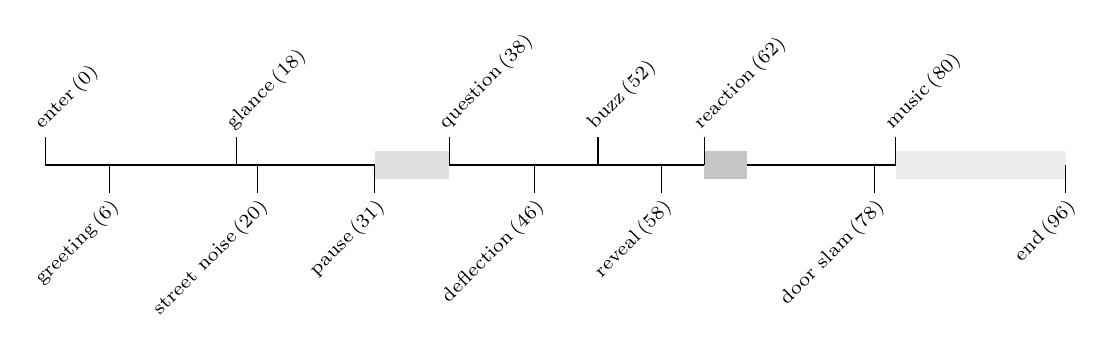
\begin{tikzpicture}[x=0.135cm, font=\scriptsize]
\draw[thick] (0,0) -- (96,0);
\fill[gray!25] (31,-0.18) rectangle (38,0.18);
\fill[gray!45] (62,-0.18) rectangle (66,0.18);
\fill[gray!15] (80,-0.18) rectangle (96,0.18);
\foreach \t/\l in {0/enter,18/glance,38/question,52/buzz,62/reaction,80/music}{
  \draw (\t,0) -- (\t,0.35);
  \node[anchor=south west, rotate=45, inner sep=1pt] at (\t,0.35) {\l\,(\t)};
}
\foreach \t/\l in {6/greeting,20/street noise,31/pause,46/deflection,58/reveal,78/door slam,96/end}{
  \draw (\t,0) -- (\t,-0.35);
  \node[anchor=north east, rotate=45, inner sep=1pt] at (\t,-0.35) {\l\,(\t)};
}
\end{tikzpicture}
\caption{Timeline of the forged-letter scene, in seconds. Shaded bands mark the pause (31 to 38), the reaction shot (62 to 66), and the music (80 to 96).}
\label{fig:timeline}
\end{figure}

Four questions about this scene recur. Which of its changes are physical movement, which are changes in what a character knows, which are changes in what the audience has been told, and which are changes in sensory intensity? Which edits of the same footage differ in pacing and which differ only in appearance? What may be altered, for instance by removing the pause or quieting the sound, without changing what matters to a viewer? And how would a person direct such a scene without specifying every movement? The bridge sections answer these in turn, each time with something more exact to observe, change, or investigate.

\section{A map of the argument}

The dependency among the parts is shown in \Cref{fig:map}. Part~I is needed throughout. Parts~II, III, and IV can be read in any order after Part~I, though the examples in Part~III use categorical language and the examples in Part~V draw on all three.

\begin{figure}[ht]
\centering
\begin{tikzpicture}[
  node distance=1.2cm and 1.6cm,
  box/.style={draw, rounded corners=2pt, minimum width=3.0cm, minimum height=0.9cm, align=center, font=\small},
  arr/.style={-{Stealth[length=2.2mm]}, thick}
]
\node[box] (I) {I. Scenario spaces\\and editing};
\node[box, below left=of I] (II) {II. Categories};
\node[box, below=of I] (III) {III. Sheaves};
\node[box, below right=of I] (IV) {IV. Types};
\node[box, below=of III] (V) {V. Generation};
\node[box, below=of V] (VI) {VI. Synthesis};
\draw[arr] (I) -- (II);
\draw[arr] (I) -- (III);
\draw[arr] (I) -- (IV);
\draw[arr] (II) -- (V);
\draw[arr] (III) -- (V);
\draw[arr] (IV) -- (V);
\draw[arr] (V) -- (VI);
\end{tikzpicture}
\caption{Dependencies among the parts of the book.}
\label{fig:map}
\end{figure}

\section{Conventions}

Mathematical objects are introduced in definitions and their basic properties are stated as propositions. Statements asserting something about cinema or perception, rather than about the mathematical model, are called principles and are not proved. A principle is a hypothesis that the model makes testable, and the text indicates in each case what would count against it.

Films are cited by title and year. Where a film is used as an example, the claim made about it concerns the model's reading of a feature the film is widely known for, such as the use of long takes or looped time, and no claim is made about the intentions of its makers.

Notation is collected in Appendix~\ref{app:notation}.

\section*{Exercises}

\begin{exercise}
Choose a sequence of three shots from a film you know well. For each of the four theoretical traditions above, state in one sentence what that tradition would take the cuts in the sequence to be doing. Identify which sentences conflict and which merely address different aspects.
\end{exercise}

\begin{exercise}
The three questions of this chapter were: what are the pieces, how do they compose, what does the composite carry. Apply them to a non-film domain, such as a proof in a textbook or a piece of chamber music, and note which of the three has the least obvious answer.
\end{exercise}
